\chapter{Functional and Non-Functional Requirements}\label{app:requirements}

The complete list of requirements, with a one-sentence summary and the prototype status of each, is kept with the source code:

\begin{center}
\url{https://github.com/rawdatarekkkk/jadwai/blob/main/docs/REQUIREMENTS.md}
\end{center}

It is derived from the project's Software Requirements Specification (SRS) v0.4 of 18 November 2026, which defines the inputs, outputs, error behaviour and acceptance criteria of every requirement. SRS v0.2 was reviewed by the supervisor; v0.3 and v0.4 carry the project owner's approval only. The status is the owner's record of the prototype on 23 November 2026, not a supervisor acceptance or a research result: \emph{implemented} means working in the prototype with automated tests, \emph{partial} that a working subset exists.

\section{Functional requirements}

Table~\ref{tab:fr-areas} groups the 78 functional requirements by area. Of these, 55 are implemented, 17 partly implemented and 6 not started.

\begin{longtable}{@{}p{0.26\textwidth}p{0.17\textwidth}p{0.155\textwidth}p{0.33\textwidth}@{}}
\caption{Functional requirements by area.}\label{tab:fr-areas}\\
\toprule
Area & Requirements & Status & Main gaps \\
\midrule
\endfirsthead
\toprule
Area & Requirements & Status & Main gaps \\
\midrule
\endhead
Term data and records & FR-001--FR-008 & Partial & One term only; no aliases or dated availability exceptions \\
Constraint vocabulary and lifecycle & FR-009--FR-013 & Partial & No supersession history or weight editing \\
AI extraction and review & FR-014--FR-023, FR-073, FR-074 & Partial & Extraction measured on development data only (Section~\ref{evidence-llm}); no audit export with cost \\
Scheduling & FR-024--FR-030, FR-065--FR-070 & Implemented & --- \\
Validation & FR-031--FR-033 & Implemented & --- \\
Scenarios and editing & FR-034--FR-039 & Partial & No explicit-variation scenarios (FR-037) \\
Publication and views & FR-040--FR-043, FR-078 & Implemented & --- \\
Export & FR-044, FR-045 & Implemented & --- \\
Traceability, accounts, audit & FR-046--FR-048 & Partial & Partial requirement-to-publication trace \\
Evaluation support & FR-049, FR-050 & Partial & No human annotations; no participant study \\
Examinations & FR-051, FR-071, FR-072 & Implemented & --- \\
Ask JAI & FR-075--FR-077 & Implemented & --- \\
Infeasibility explanation & FR-058 & Implemented & --- \\
Extensions & FR-052--FR-057 & Mostly not started & Arabic extraction (FR-054) works but is unmeasured \\
Exception handling & FR-059--FR-064 & Partial & Cancelled results are not retained \\
\bottomrule
\end{longtable}

\section{Non-functional requirements}

The SRS defines 23 non-functional requirements and invents no numeric targets; values that depend on later decisions remain open. Table~\ref{tab:nfr} summarises them.

\begin{longtable}{@{}p{0.19\textwidth}p{0.17\textwidth}p{0.56\textwidth}@{}}
\caption{Non-functional requirements and prototype status.}\label{tab:nfr}\\
\toprule
Category & Requirements & Status \\
\midrule
\endfirsthead
\toprule
Category & Requirements & Status \\
\midrule
\endhead
Correctness & NFR-001--003 & Met in tests: separate validator; publication refused on any violation; a time limit is never reported as infeasibility \\
Security & NFR-004, 005 & Server-side permissions; no secrets in the repository. Passwords use scrypt instead of the specified Argon2id (recorded deviation) \\
Privacy & NFR-006, 007 & With the local model no text leaves the server; applicable data-protection rules still to be confirmed \\
Accessibility & NFR-008 & Labelled, keyboard-operable controls; no formal audit \\
Reliability & NFR-009, 010 & Timeouts, retries, malformed output and cancellation tested; recovery objectives open \\
Performance and scale & NFR-011--013 & Runtime, outcome and tested scale recorded with every result; no numeric targets \\
Usability & NFR-014, 015 & Checked manually; not measured (no participant study) \\
Reproducibility & NFR-016 & Versions, seeds and dates recorded for runs and fine-tuning \\
Maintainability & NFR-017 & Separate modules; model provider chosen by configuration \\
Compatibility, retention, backup & NFR-018--020 & Open; local backups before destructive changes \\
Localisation & NFR-021 & English and Arabic interface with right-to-left layout; mixed Arabic/English text kept in reading order \\
Observability, licensing & NFR-022, 023 & Partial; licence list not yet checked \\
\bottomrule
\end{longtable}

\chapter{Screenshots of the Prototype}\label{app:screenshots}

The following screenshots were taken from the running prototype on 23 November 2026 in the demonstration workspace (a browser window of 1440$\times$900 pixels). All names of people are demonstration placeholders. Further screenshots are in the repository folder \texttt{docs/screenshots}.

\begin{figure}[p]
\centering
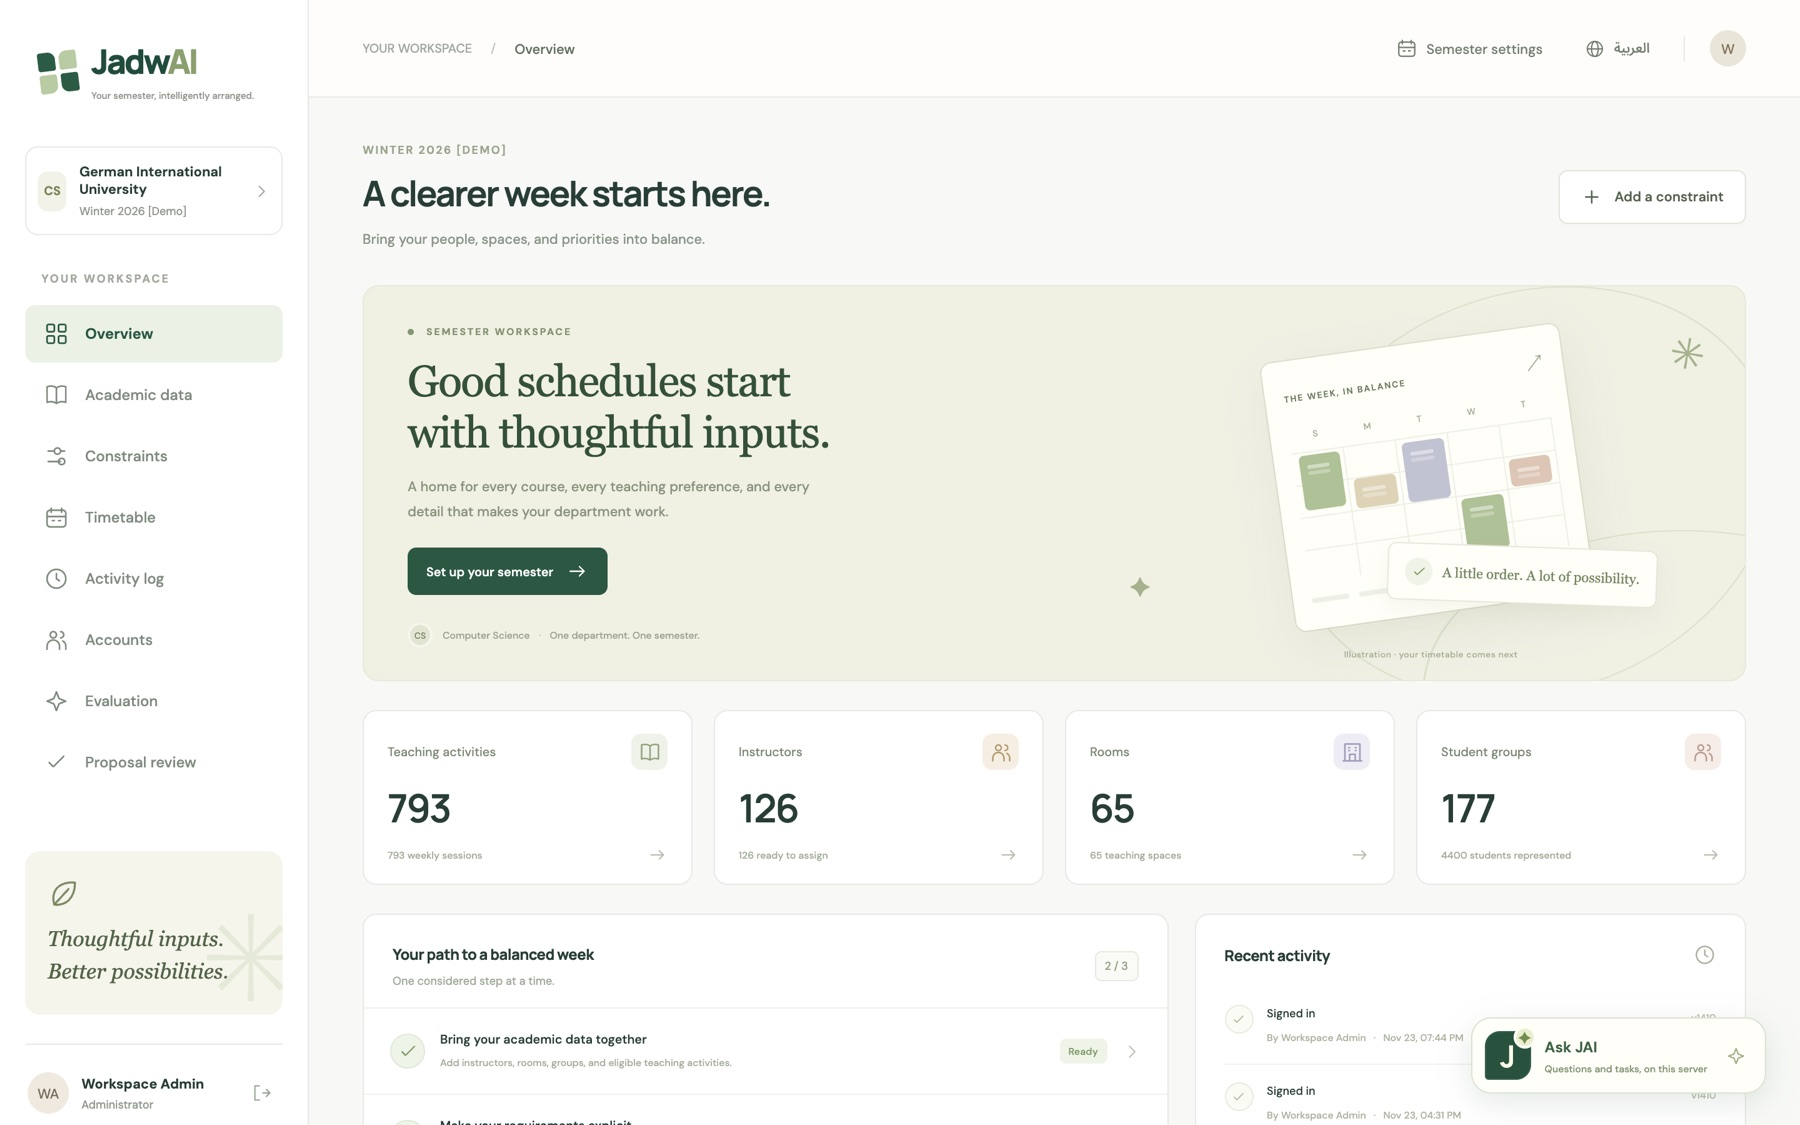
\includegraphics[width=\textwidth]{02-overview.jpg}
\caption{Overview page of the administrator workspace: counts of activities, instructors, rooms and student groups, the setup path and recent activity.}
\label{fig:shot-overview}
\end{figure}

\begin{figure}[p]
\centering
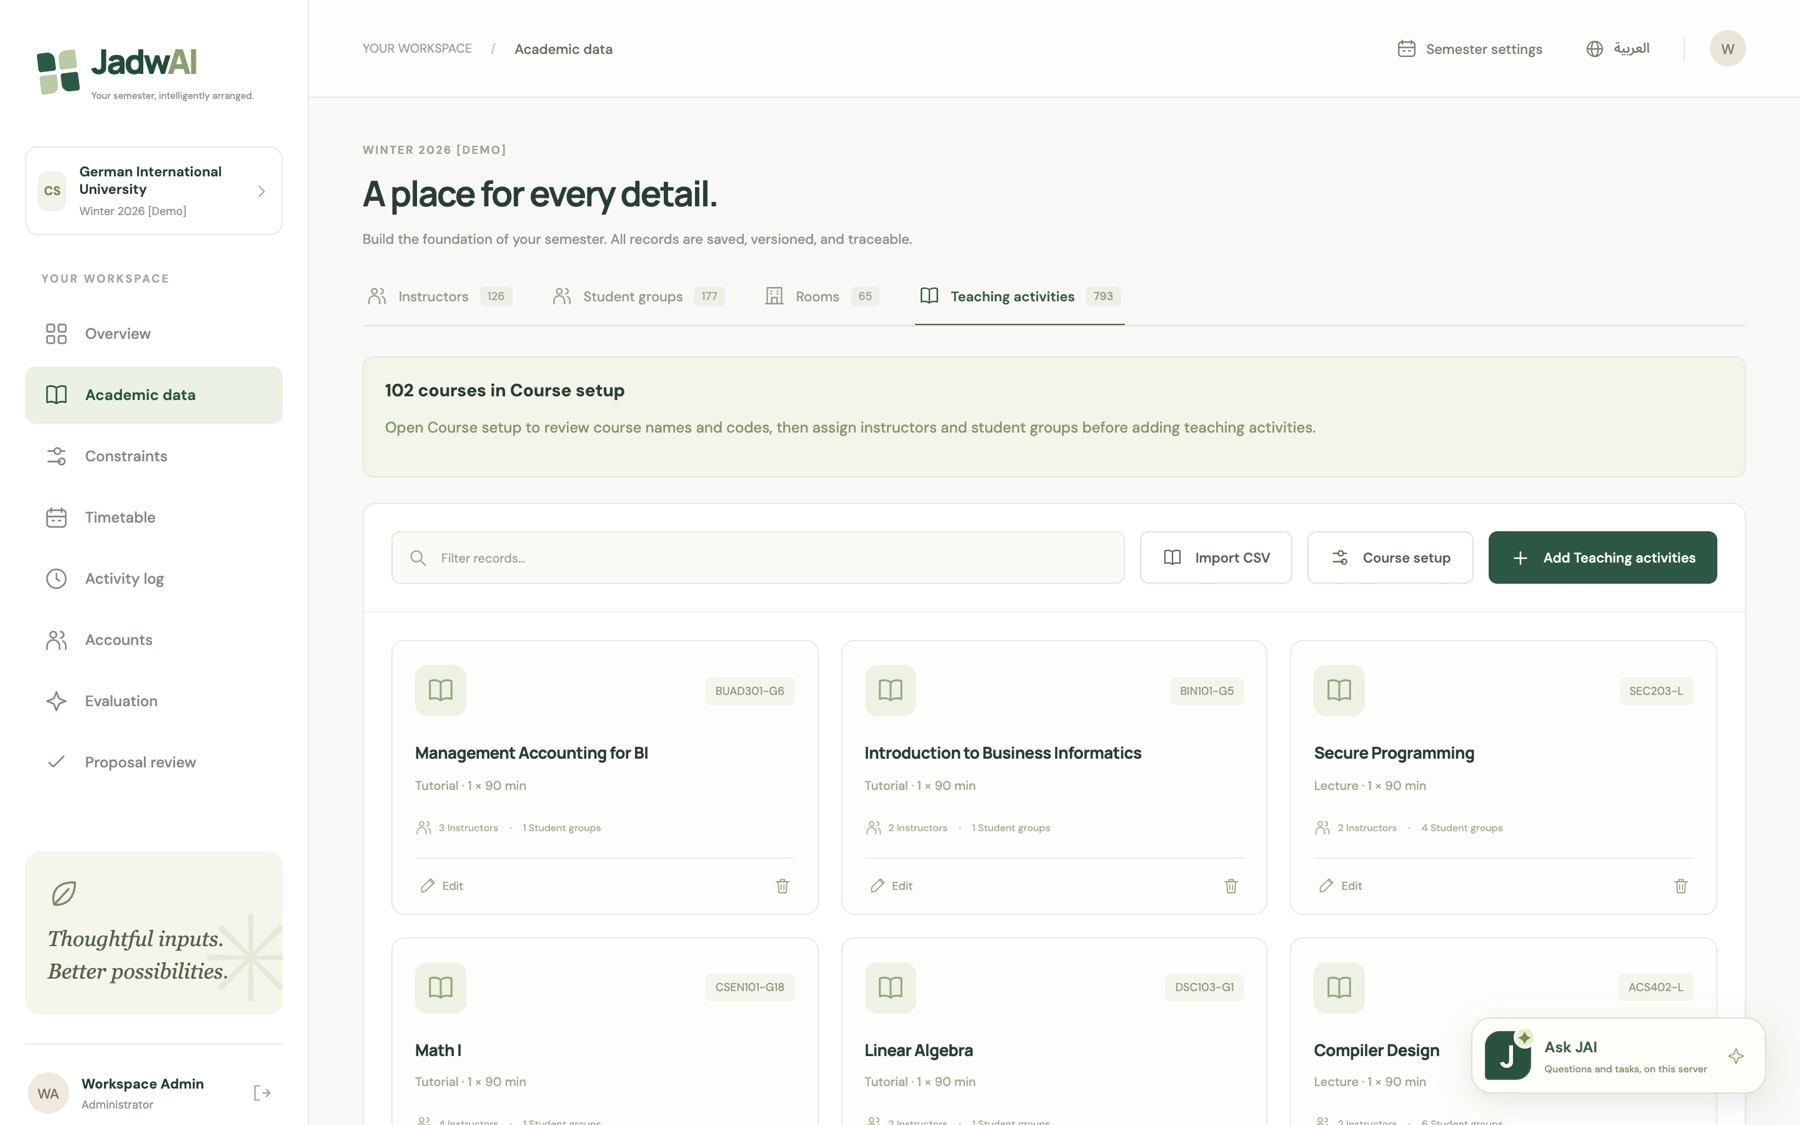
\includegraphics[width=\textwidth]{03-academic-data.jpg}
\caption{Academic data: teaching activities of each course, with separate tabs for instructors, student groups and rooms, and CSV import.}
\label{fig:shot-academic-data}
\end{figure}

\begin{figure}[p]
\centering
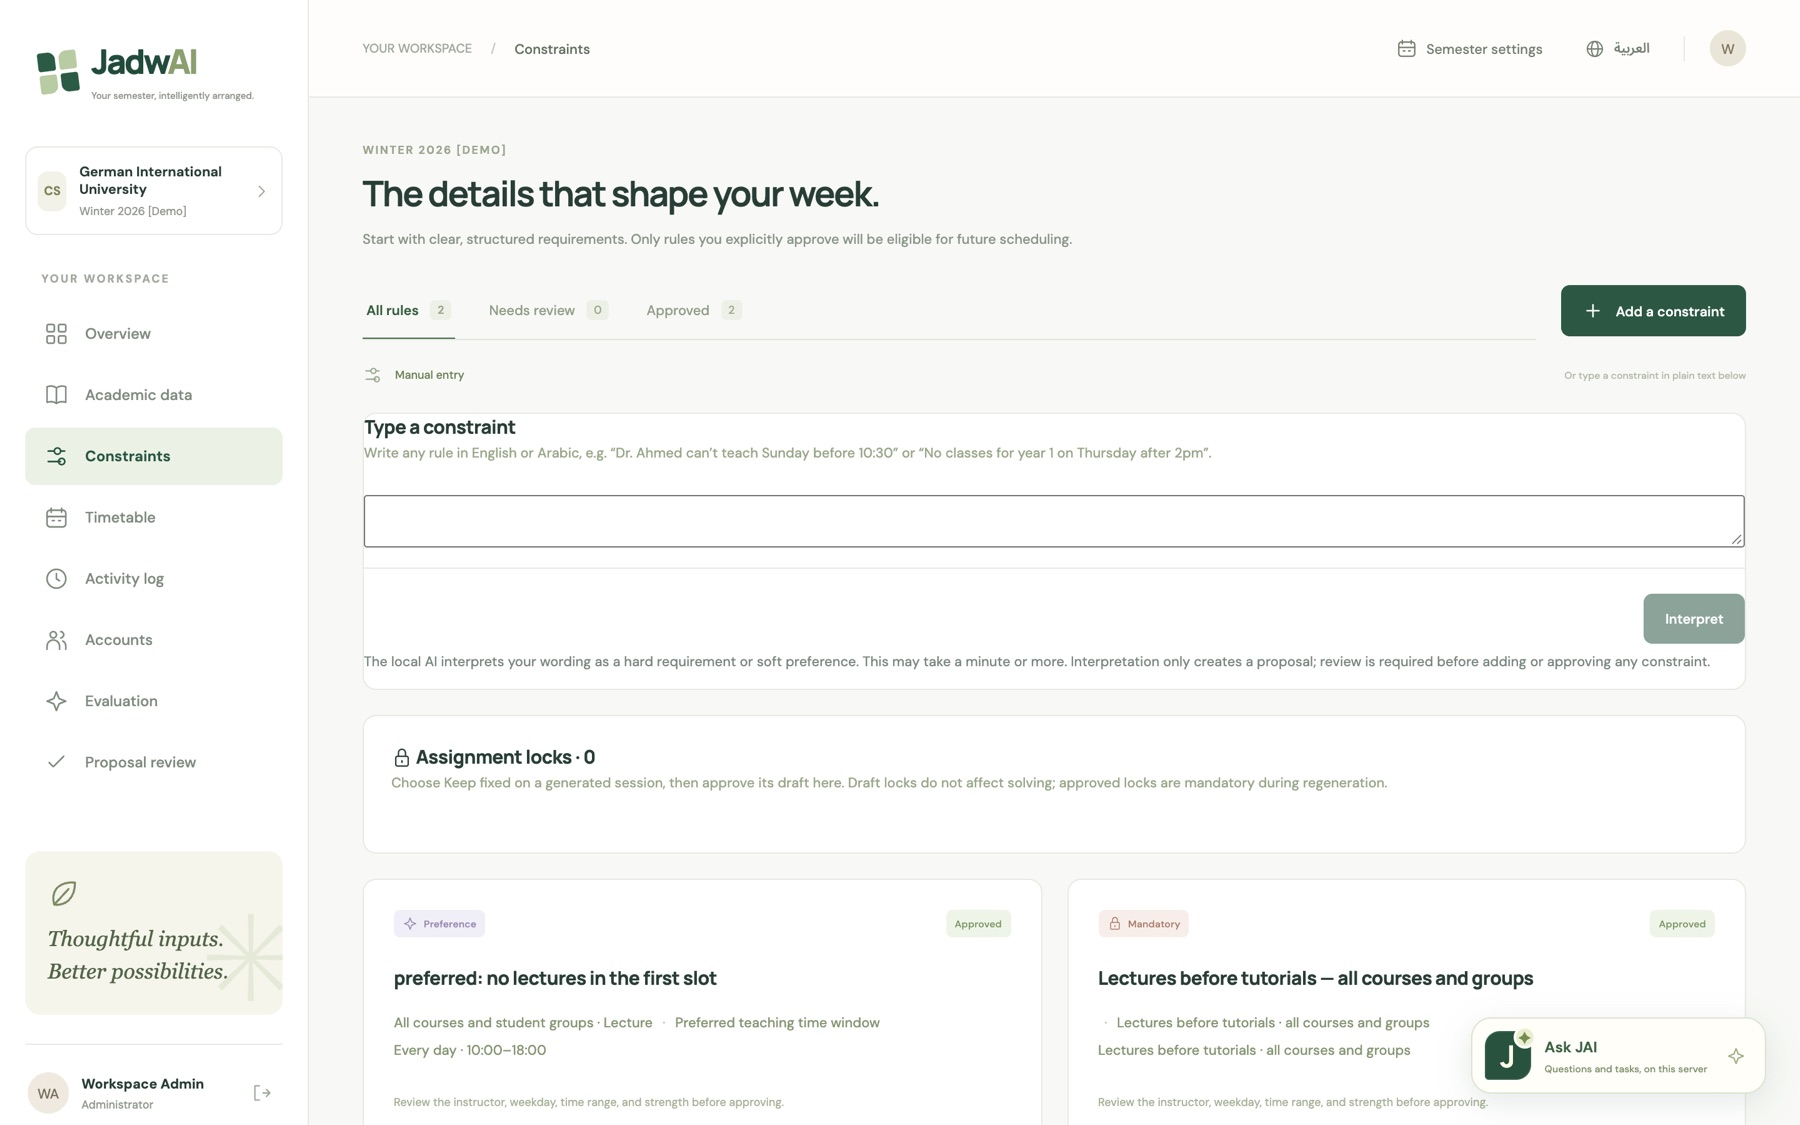
\includegraphics[width=\textwidth]{04-constraints.jpg}
\caption{Constraints: a requirement can be typed in English or Arabic and is interpreted as a proposal; approved rules are listed below with their strength (preference or mandatory).}
\label{fig:shot-constraints}
\end{figure}

\begin{figure}[p]
\centering
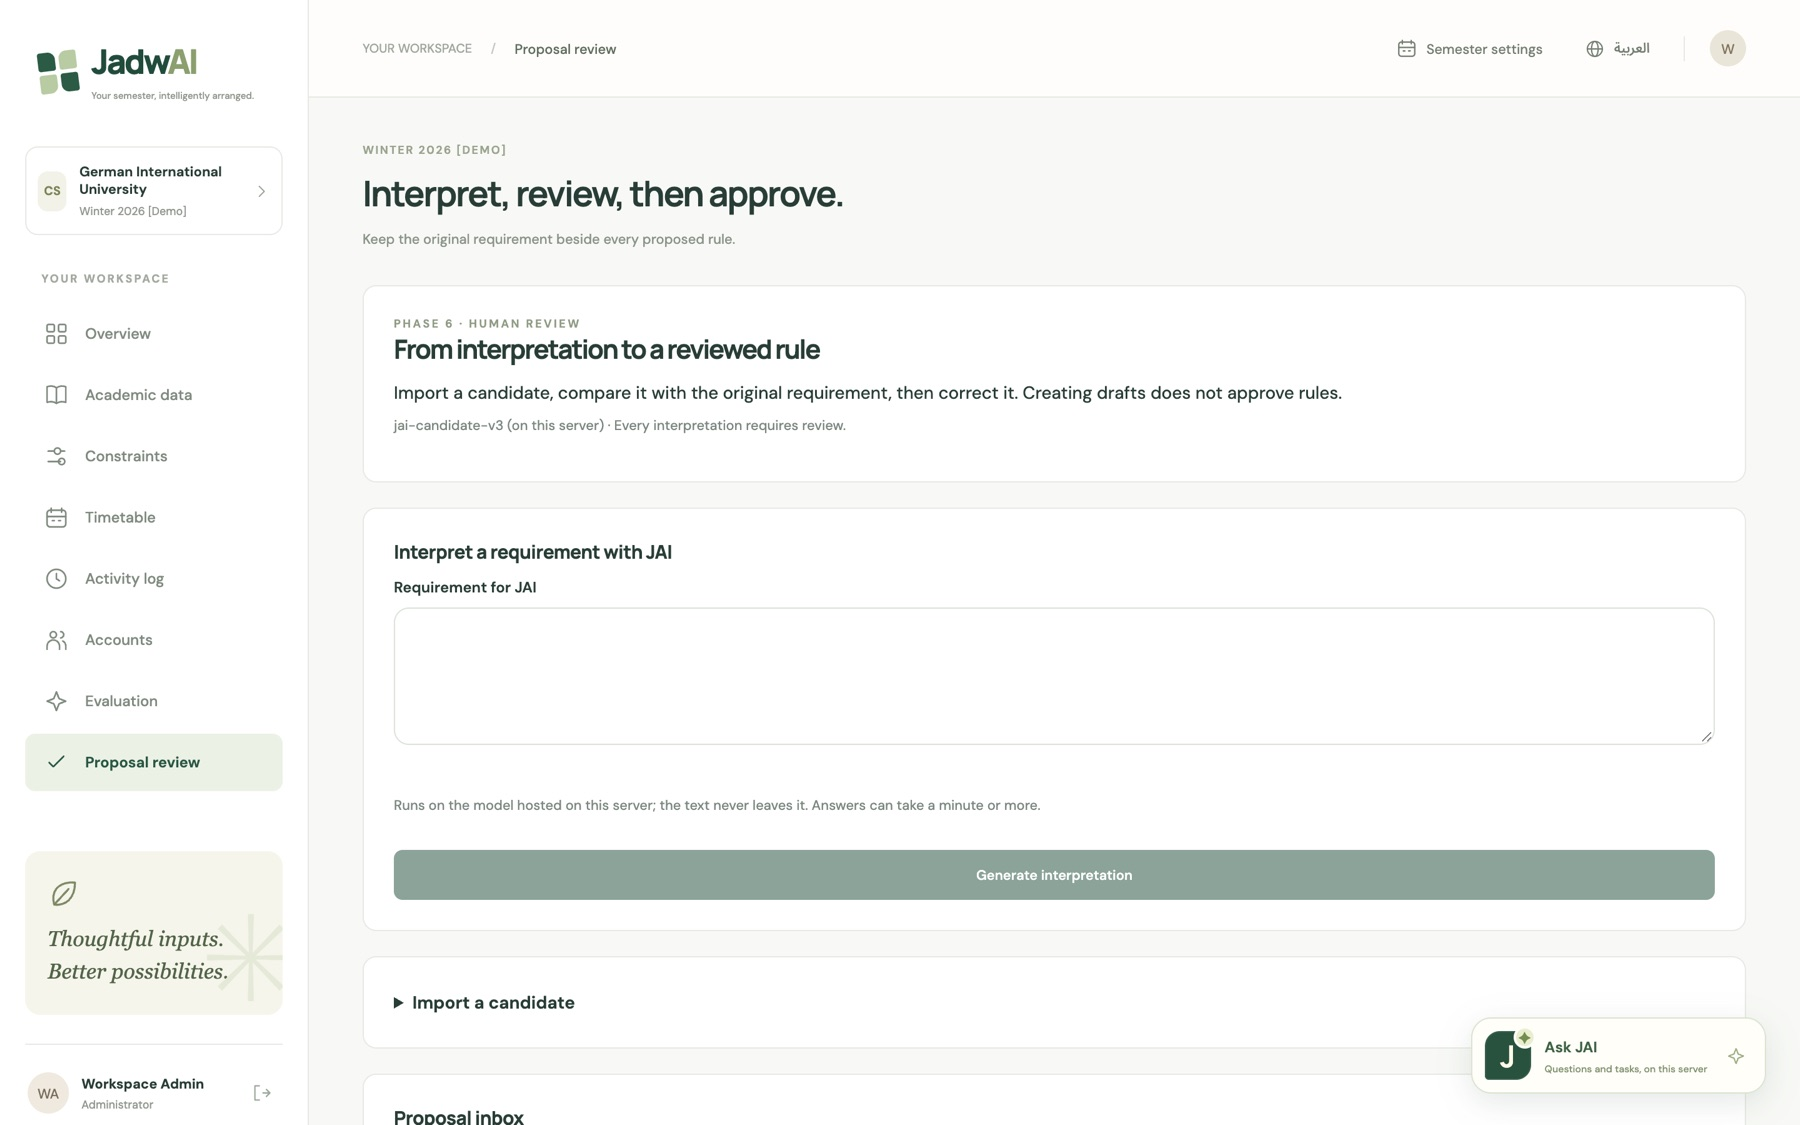
\includegraphics[width=\textwidth]{09-proposal-review.jpg}
\caption{Proposal review: a requirement is interpreted by the locally hosted model and shown beside the original text for correction before any rule is created.}
\label{fig:shot-proposal-review}
\end{figure}

\begin{figure}[p]
\centering
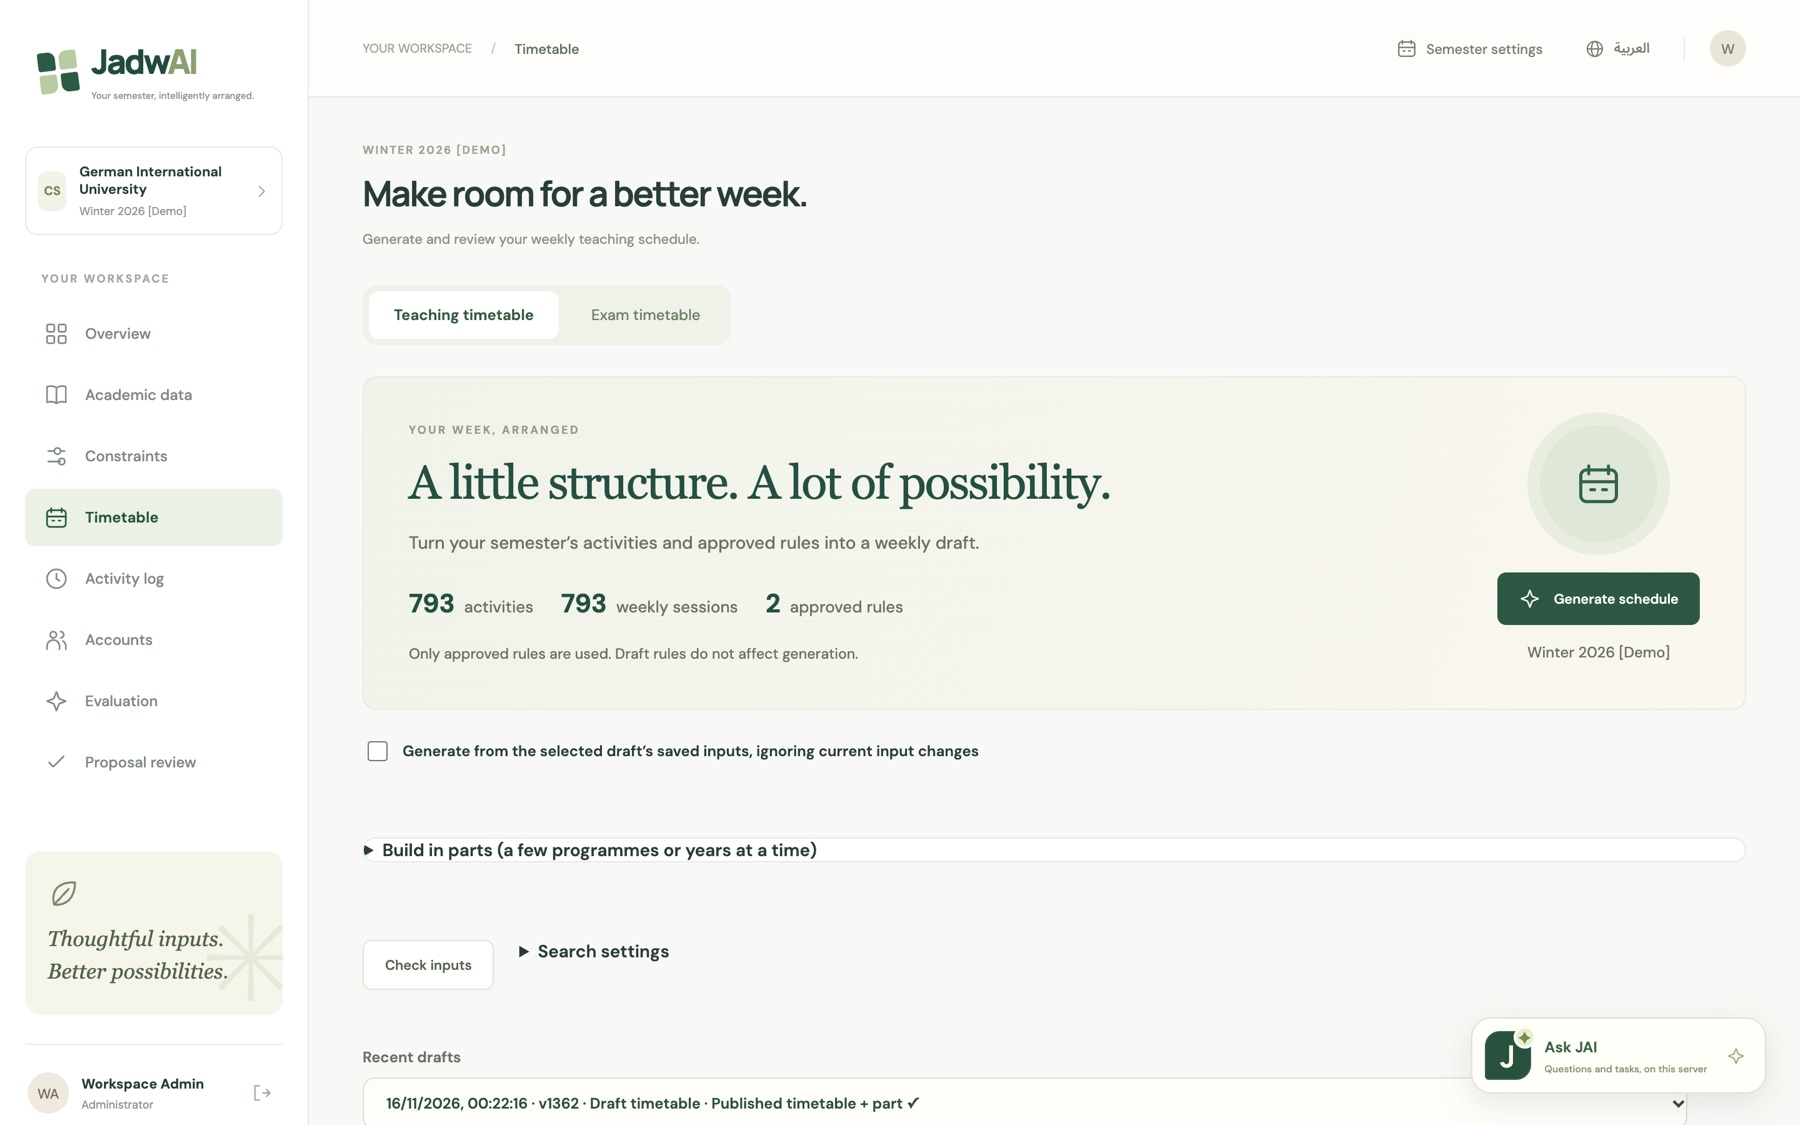
\includegraphics[width=\textwidth]{13-teaching-timetable-top.jpg}
\caption{Teaching timetable: generation from approved rules only, building in parts, input checks, search settings and the list of saved drafts.}
\label{fig:shot-teaching-timetable-top}
\end{figure}

\begin{figure}[p]
\centering
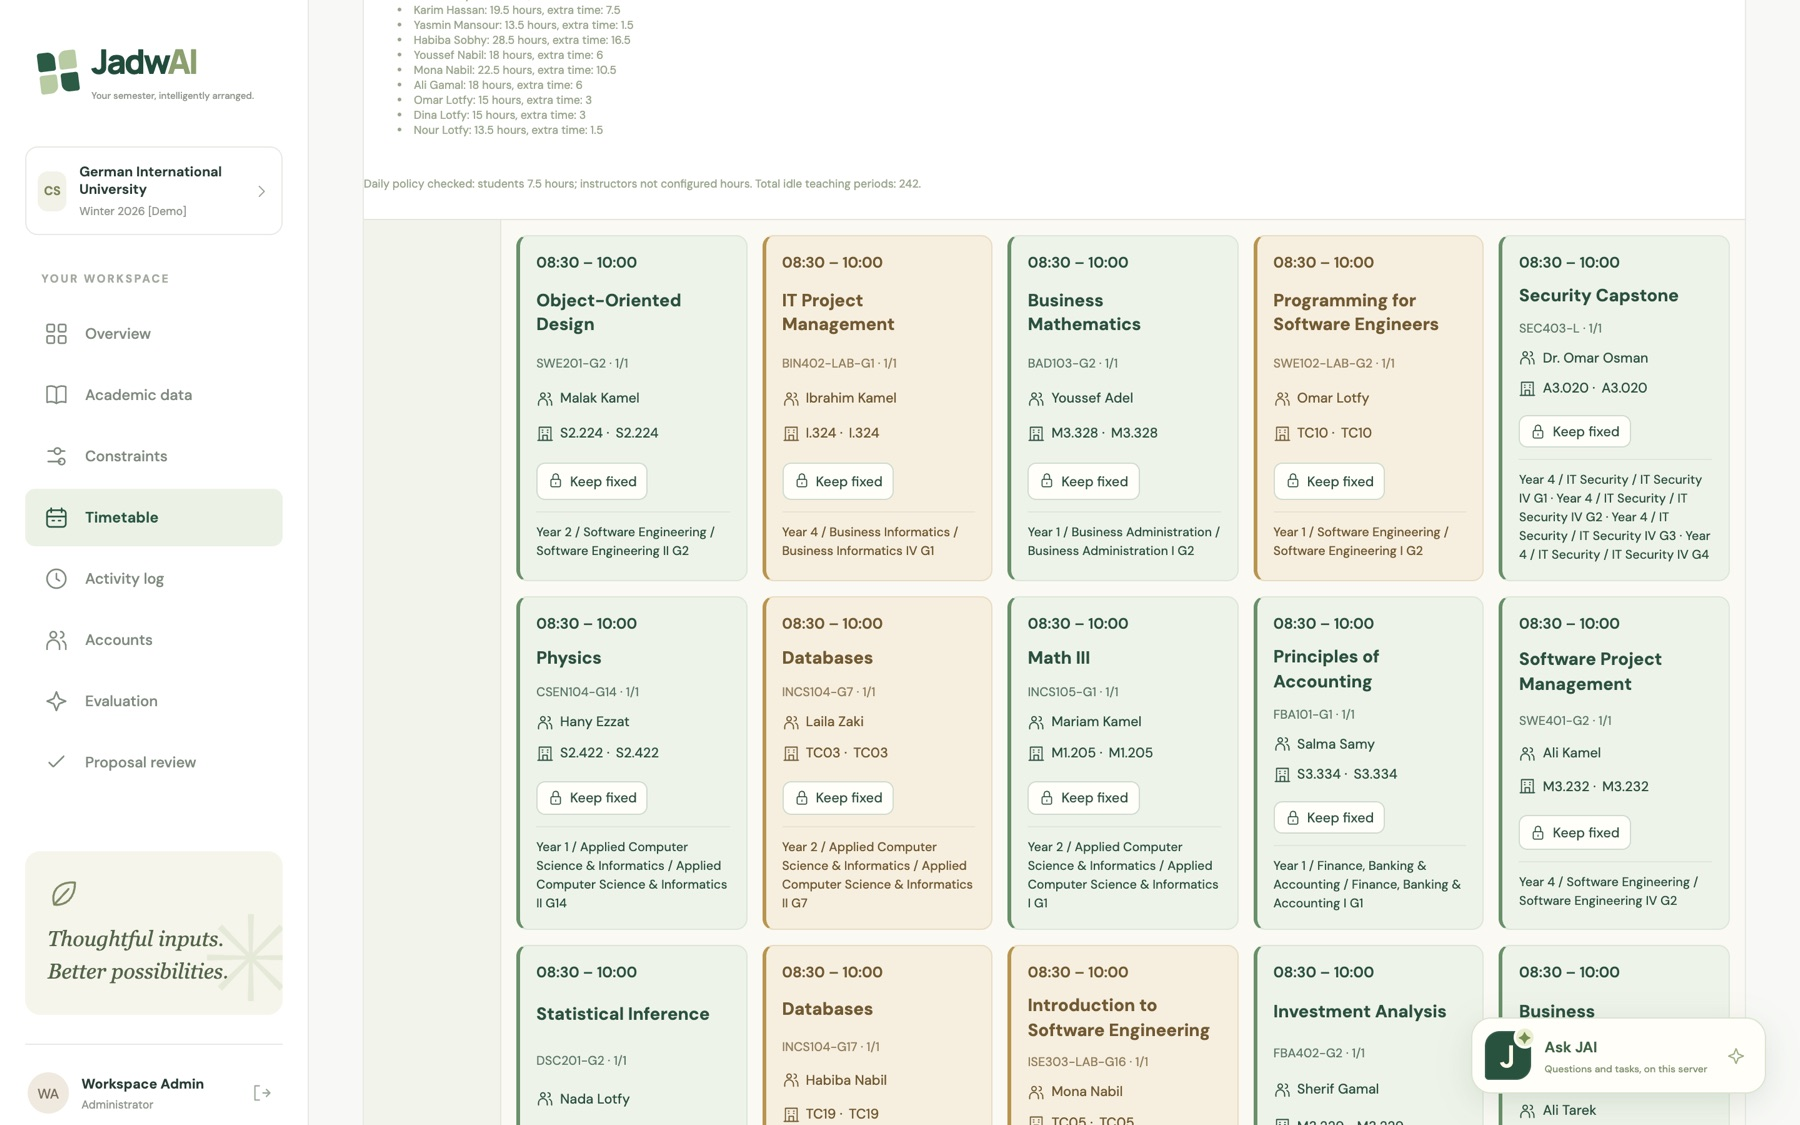
\includegraphics[width=\textwidth]{15-teaching-timetable-2.jpg}
\caption{Part of a published teaching timetable: each session shows time, course, activity, instructor and room, with an option to keep it fixed in later regenerations.}
\label{fig:shot-teaching-timetable-2}
\end{figure}

\begin{figure}[p]
\centering
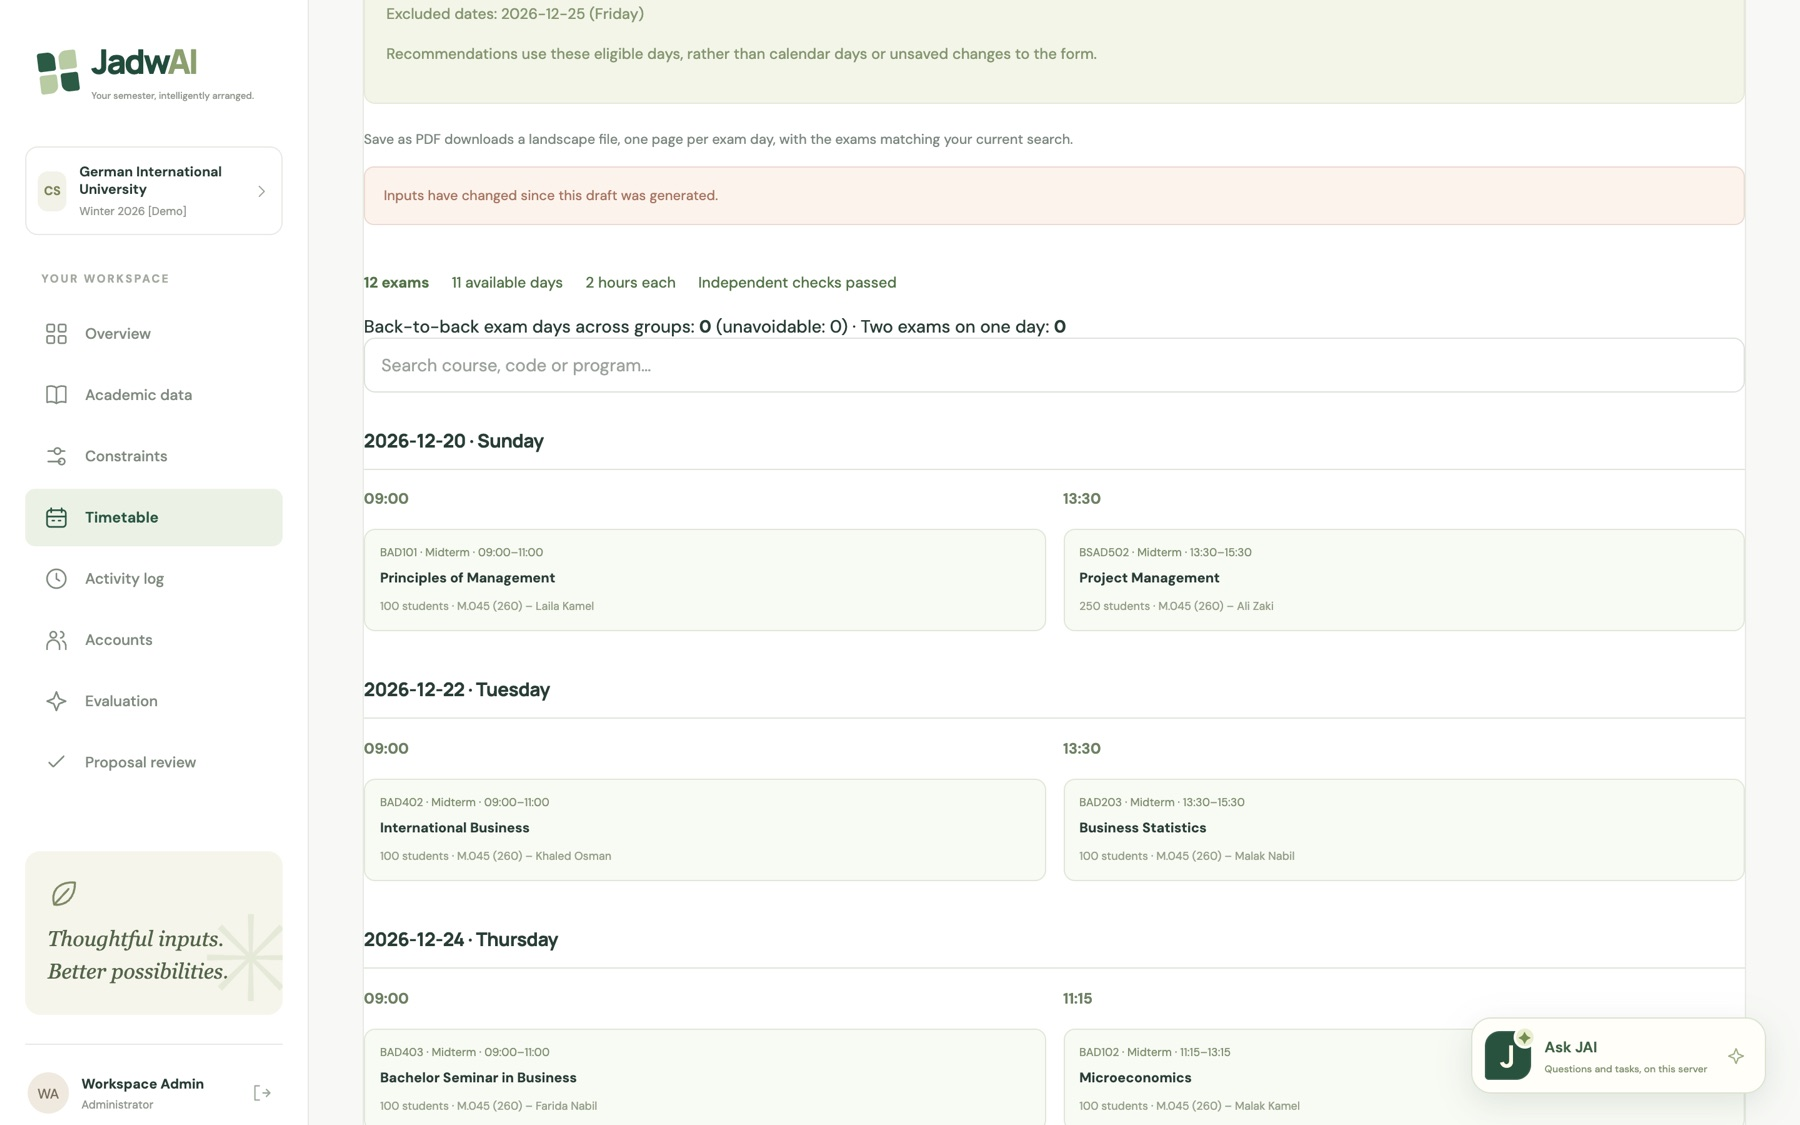
\includegraphics[width=\textwidth]{16-exam-timetable.jpg}
\caption{Examination timetable: midterms by day and time with hall, capacity and invigilator; the summary reports back-to-back examination days across groups.}
\label{fig:shot-exam-timetable}
\end{figure}

\begin{figure}[p]
\centering
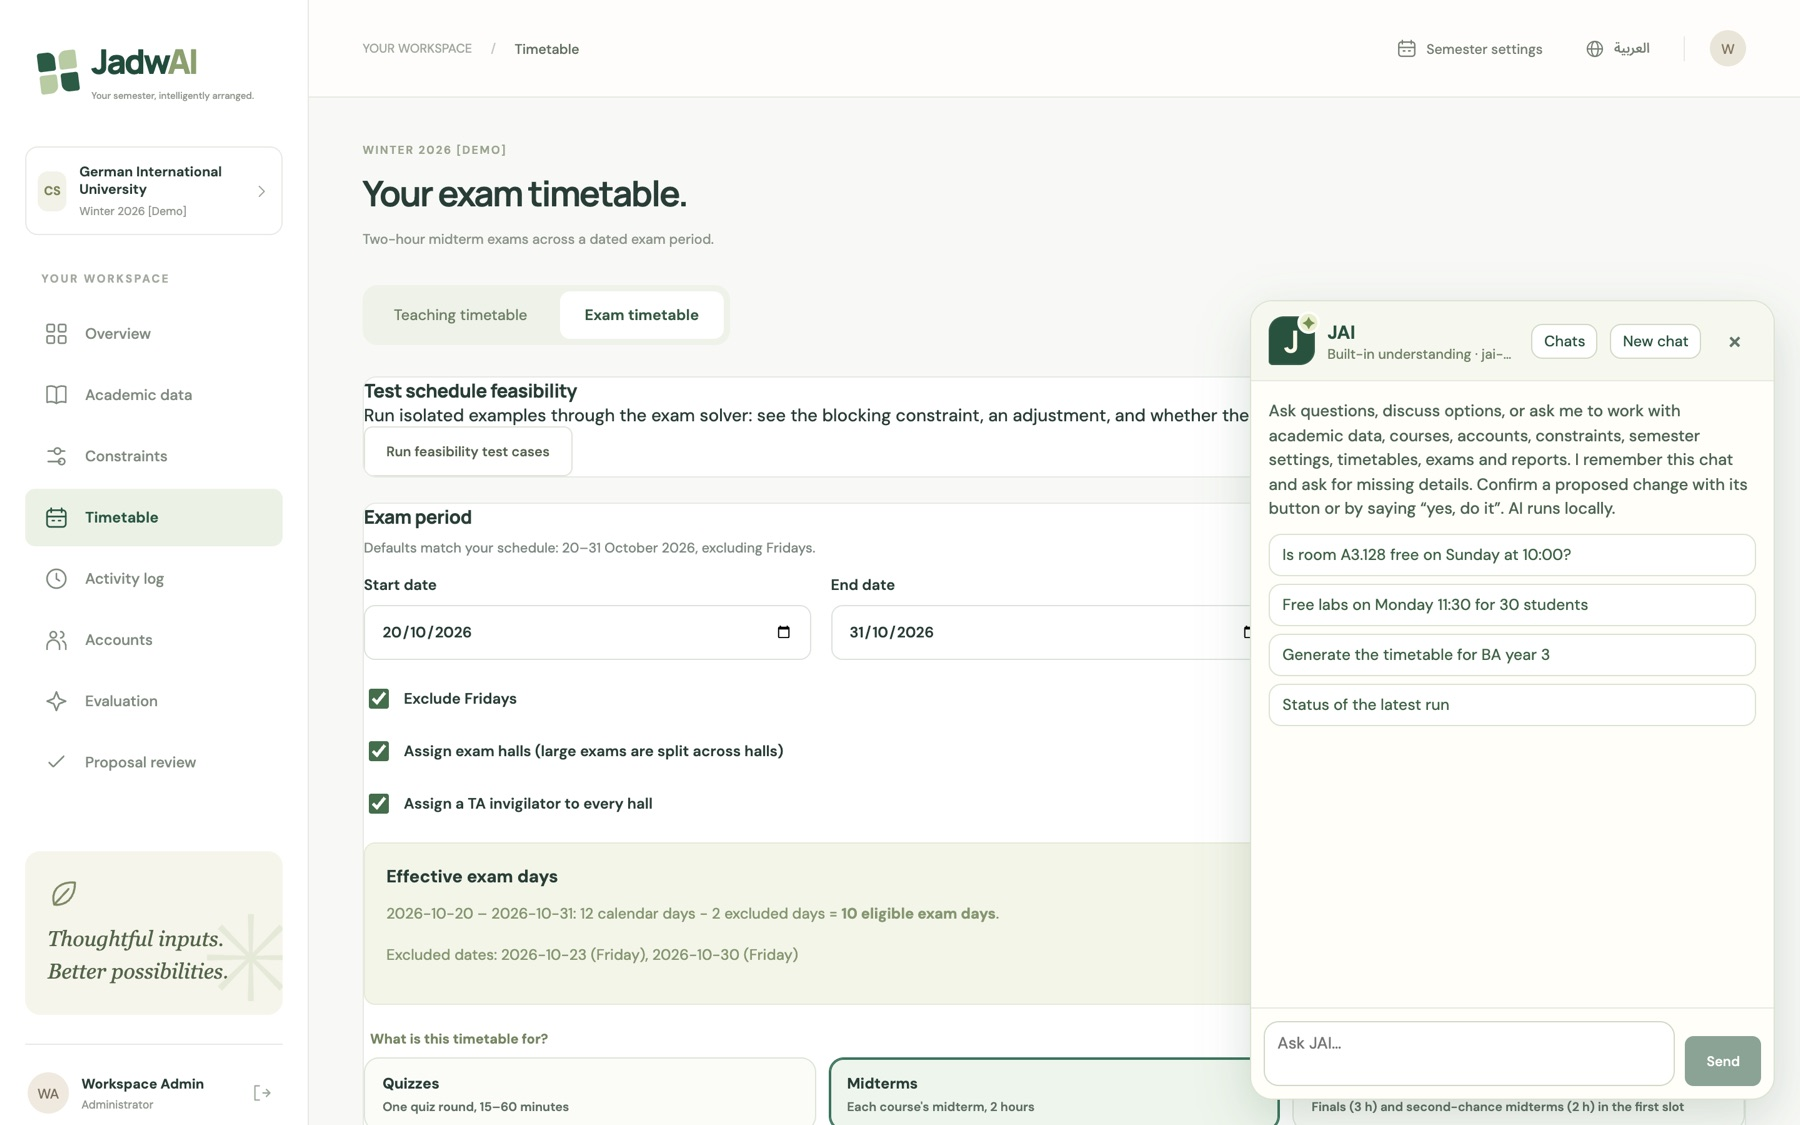
\includegraphics[width=\textwidth]{18-jai-chat.jpg}
\caption{The JAI chat panel beside the exam settings: example questions and tasks; a proposed change runs only after the administrator confirms it.}
\label{fig:shot-jai-chat}
\end{figure}

\begin{figure}[p]
\centering
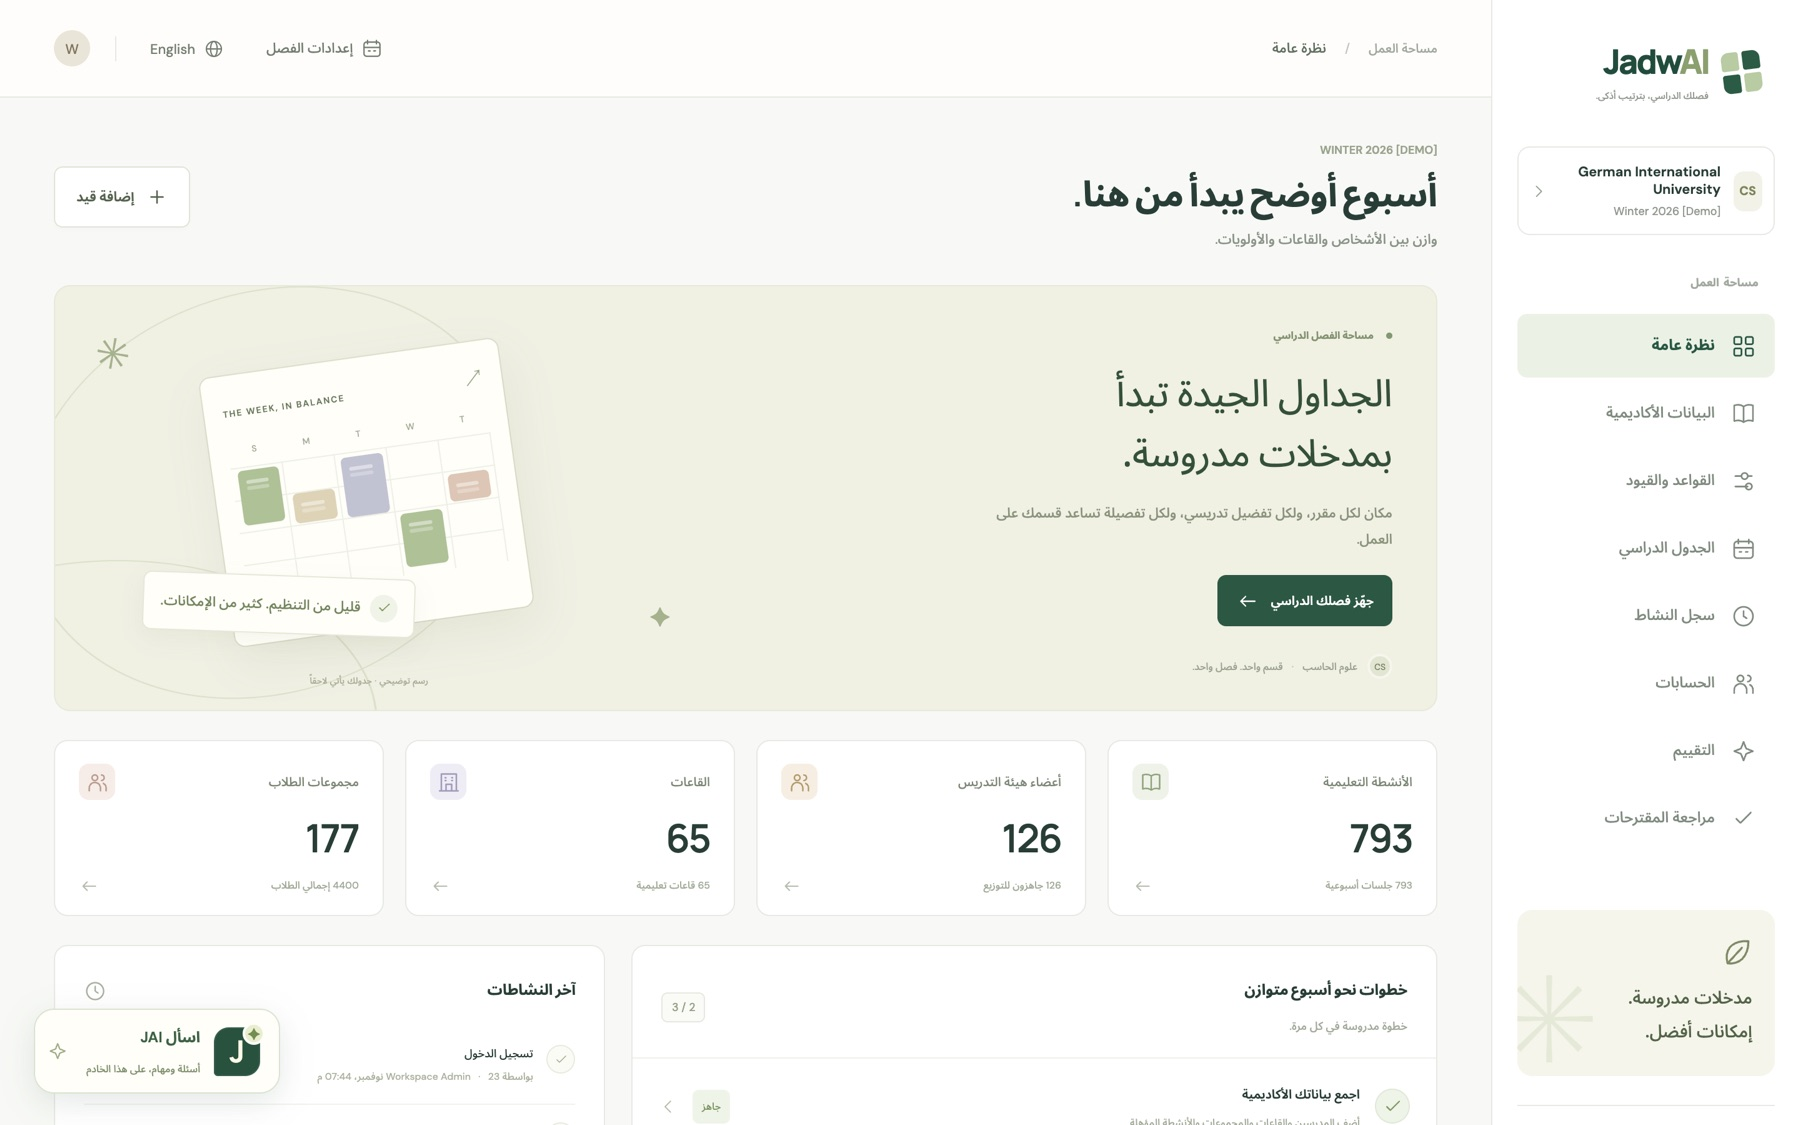
\includegraphics[width=\textwidth]{11-overview-arabic.jpg}
\caption{Arabic interface: the same overview page with right-to-left layout.}
\label{fig:shot-overview-arabic}
\end{figure}

\begin{figure}[p]
\centering
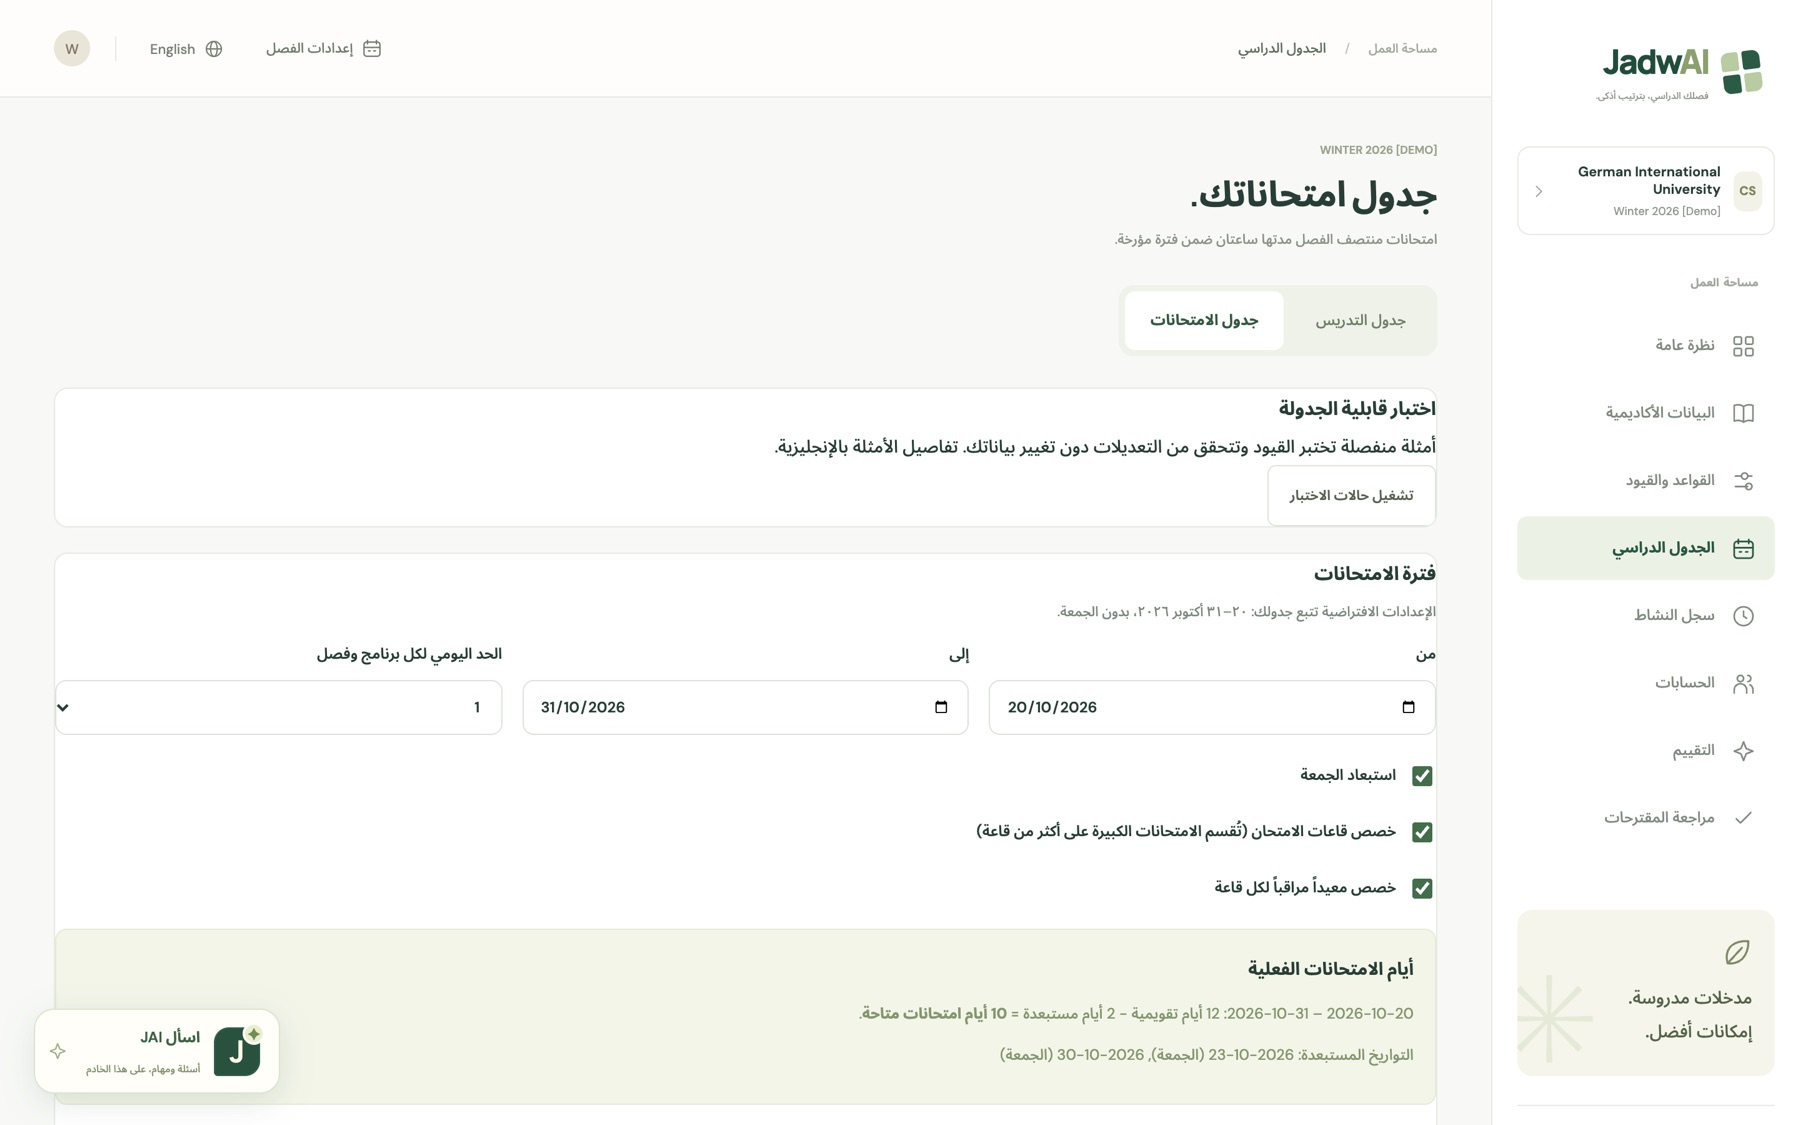
\includegraphics[width=\textwidth]{12-timetable-arabic.jpg}
\caption{Arabic interface: the examination settings page.}
\label{fig:shot-timetable-arabic}
\end{figure}

\clearpage

\chapter{Project Record and Traceability}\label{app:planning}

% NOTE (24 Nov 2026): Replaces the October planning records (timeline without dates, proposed deliverables, open decisions). Drafted with AI assistance; reword in your own words. Dates come from the SRS versions, the corpus manifests, finetuning/RESULTS.md and the git history.

\section{Timeline}\label{timeline}

Table~\ref{tab:timeline} lists the main milestones of the project as they happened.

\begin{longtable}[]{@{}p{0.24\textwidth}p{0.68\textwidth}@{}}
\caption{Project milestones.}\label{tab:timeline}\\
\toprule
Date (2026) & Milestone \\
\midrule
\endhead
\bottomrule
\endlastfoot
10 October & SRS draft v0.2 reviewed by the supervisor \\
25 October & Synthetic corpus release \texttt{0.1.0-draft} (128 statements) and annotation guide v1 \\
1 November & Development bundle \texttt{0.2.0-draft} (144 statements, two contexts) and annotation guide v2 \\
4--8 November & Examination halls and invigilators, scenarios and publication, portals, advising students, generation in parts, repair suggestions \\
8 November & Measured evidence for Chapter~\ref{evidence} (department and university scale, repair, rule-based baseline) \\
12 November & Examination plans with quizzes, midterms, finals and second chances \\
14--18 November & JAI chat: built-in answers, local model, confirmed tasks; SRS v0.4 \\
19--23 November & JAI fine-tuning rounds 1--3, verified guide, blind rating, Arabic reply and display fixes \\
23--24 November & Fine-tuning round 4 and its blind rating; two local-model extraction runs on the development corpus; examination publishing as a built-in chat route; annotation guide v2.1 merges two pairs of synonymous codes; thesis moved to the GIU template \\
10 December & Full draft due to the supervisor \\
\end{longtable}

\section{Deliverables}\label{proposed-deliverables-of-the-study}

\begin{itemize}
\item The JadwAI prototype (\texttt{frontend/}, \texttt{backend/}, \texttt{worker/}) with its automated tests.
\item The requirements with their status (\texttt{docs/REQUIREMENTS.md}, summarised in Appendix~\ref{app:requirements}).
\item The output contract, annotation guides, synthetic corpus and offline scorer (\texttt{evaluation/}).
\item The fine-tuning data, training notebook, merge and evaluation tools, and results (\texttt{finetuning/}).
\item The scripts, logs, predictions and scores behind every reported measurement, in \texttt{thesis/evidence/}.
\item This thesis.
\end{itemize}

\section{Traceability to the requirements}\label{consistency-with-the-srs-traceability}

Table~\ref{tab:trace} links each part of the method in Chapter~\ref{methodology-proposed-study} to the functional requirements it relies on.

\begin{longtable}[]{@{}p{0.5\textwidth}p{0.42\textwidth}@{}}
\caption{Traceability of the method to the requirements.}\label{tab:trace}\\
\toprule
Element of the method & Requirement or procedure \\
\midrule
\endhead
\bottomrule
\endlastfoot
Schema-constrained interpretation & FR-015, FR-022, FR-074 \\
Entity resolution without invented entities & FR-016 \\
Parameters and named periods & FR-001, FR-017, FR-067 \\
Negation and mandatory/preferred strength & FR-018 \\
Clarification and unsupported requests & FR-019 \\
Review beside the original statement & FR-020 \\
Approval gate before generation & FR-021 \\
Rule-based parser compared with the model & FR-073 \\
Four language categories & FR-054 \\
Corpus, scorer and development records & FR-049 \\
Manual entry (forms) & FR-010 \\
Manual versus assisted entry with participants & FR-050 (not carried out) \\
Scheduling measures & FR-024--FR-029, FR-031 \\
Validator checks, coverage and publication gate & FR-030--FR-033, FR-040, FR-063 \\
Repair suggestions & FR-058 \\
Examination timetables & FR-051, FR-071, FR-072 \\
JAI assistant and its evaluation & FR-075--FR-077 \\
Reproducibility records & FR-023--FR-025; NFR-016 \\
Comparison of validator and solver model & NFR-002 (research procedure) \\
Annotator agreement and confidence intervals & Research procedure, no FR \\
\end{longtable}
